\documentclass[aspectratio=169]{beamer}
\usetheme{Hannover}
\usepackage{graphicx}
\usepackage{wrapfig}
\usepackage{multimedia}
%%%%%%%%%%%%%%%%%%%%%%%%%%%%%%%%%
\section{Introduction}
\subsection{My Research Topic}
%%%%%%%%%%%%%%%%%%%%%%%%%%%%%%%%%
\begin{document}
\begin{frame}
\frametitle{My Research Topic}
During my MRes course, I plan to research the influence of Korean Pop (Kpop) within Japan.
\newline
You can find advertisements for Kpop all around Tokyo, but where is the research on this phenomenon?
\newline
\begin{figure}[h]

\includegraphics[scale=0.2]{bts}
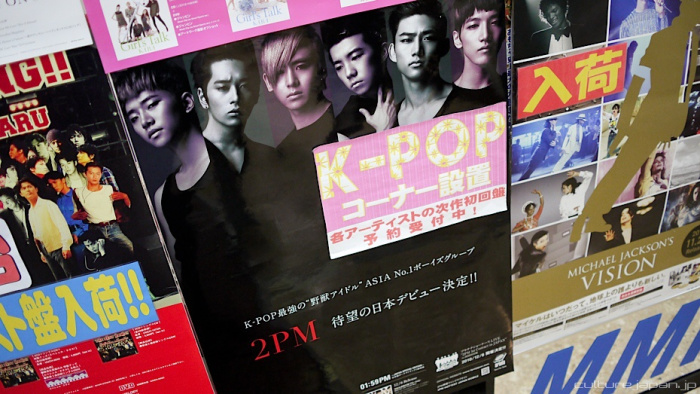
\includegraphics[scale=0.6]{kpopexample}
\end{figure}
\end{frame}
%%%%%%%%%%%%%%%%%%%%%%%%%%%%%%%%%%
\subsection{Data Analysis in R}
%%%%%%%%%%%%%%%%%%%%%%%%%%%%%%%%%%
\begin{frame}
\frametitle{Data Analysis in R}
%include font and spacing?%
I used R to form a code line that could analyse specific groups of responses out of the thousands I could receive from an online survey.
R allows me to:
\begin{itemize}
\item Immediately take online responses from surveys
\item Input them into a well-structured database
\item Select specific groups within the database
\item Create graphs of my data
\end{itemize}
With this tool chain, I am well-prepared to start my research in the months to come!
 \end{frame}
 \end{document}